\documentclass[a4paper,12pt]{article}

% ======================================================================
% PACKAGES
% ======================================================================
\usepackage[utf8]{inputenc}
\usepackage[T1]{fontenc}
\usepackage{amsmath,amssymb}
\usepackage{array}
\usepackage{booktabs}
\usepackage{geometry}
\usepackage{parskip}
\usepackage{enumitem}
\usepackage{caption}
\usepackage{hyperref}
\usepackage{tabularx}
\usepackage{multirow}
\usepackage{xcolor}
\usepackage[most]{tcolorbox}
\usepackage{float}
\usepackage{siunitx}
\usepackage{graphicx}
\usepackage{tikz}
\usetikzlibrary{arrows.meta,positioning,shapes.geometric,calc}

\geometry{margin=2.5cm}

\hypersetup{
    colorlinks=true,
    linkcolor=blue!60!black,
    urlcolor=blue!60!black,
    citecolor=blue!60!black
}

\setlist[itemize]{topsep=3pt,itemsep=2pt,parsep=0pt}
\setlist[enumerate]{topsep=3pt,itemsep=2pt,parsep=0pt}
\captionsetup{font=small,labelfont=bf}

\newcolumntype{Y}{>{\raggedright\arraybackslash}X}

% ======================================================================
% BOX STYLES
% ======================================================================
\newtcolorbox{notebox}[1][]{
    enhanced,
    colback=blue!4!white,
    colframe=blue!55!black,
    fonttitle=\bfseries,
    title=#1,
    boxrule=0.6pt,
    arc=2mm,
    left=2mm,right=2mm,top=1mm,bottom=1mm
}

\newtcolorbox{warnbox}[1][]{
    enhanced,
    colback=orange!5!white,
    colframe=orange!65!black,
    fonttitle=\bfseries,
    title=#1,
    boxrule=0.6pt,
    arc=2mm,
    left=2mm,right=2mm,top=1mm,bottom=1mm
}

\newtcolorbox{keybox}[1][]{
    enhanced,
    colback=green!4!white,
    colframe=green!45!black,
    fonttitle=\bfseries,
    title=#1,
    boxrule=0.6pt,
    arc=2mm,
    left=2mm,right=2mm,top=1mm,bottom=1mm
}

\newtcolorbox{calcbox}[1][]{
    enhanced,
    colback=purple!4!white,
    colframe=purple!55!black,
    fonttitle=\bfseries,
    title=#1,
    boxrule=0.6pt,
    arc=2mm,
    left=2mm,right=2mm,top=1mm,bottom=1mm
}

\newtcolorbox{errbox}[1][]{
    enhanced,
    colback=red!4!white,
    colframe=red!60!black,
    fonttitle=\bfseries,
    title=#1,
    boxrule=0.6pt,
    arc=2mm,
    left=2mm,right=2mm,top=1mm,bottom=1mm
}

% ======================================================================
% TIKZ STYLES
% ======================================================================
\tikzset{
    workflowbox/.style={
        rectangle,
        rounded corners,
        draw=#1!70!black,
        fill=#1!8!white,
        thick,
        align=center,
        text width=2.8cm,
        minimum height=1.65cm,
        inner sep=4pt
    },
    smallworkflowbox/.style={
        rectangle,
        rounded corners,
        draw=#1!70!black,
        fill=#1!8!white,
        thick,
        align=center,
        text width=2.6cm,
        minimum height=1.45cm,
        inner sep=3pt
    },
    workflowarrow/.style={
        -{Latex[length=2mm]},
        thick,
        draw=black!65
    },
    feedbackarrow/.style={
        -{Latex[length=2mm]},
        thick,
        dashed,
        draw=black!55
    }
}

% ======================================================================
% TITLE
% ======================================================================
\title{\textbf{RSE3010: Mine Geotechnical Engineering}\\Week 3 Study Notes}
\author{Monash University, Semester 1, 2026}
\date{Based on Week 3 Lecture Slides}

\begin{document}

\maketitle

% ======================================================================
\section{Week 3: Rock Mass Classification -- RMR, Q-System \& GSI}
% ======================================================================

\subsection{Purpose}

To understand and apply the most widely used rock mass classification systems:
Rock Mass Rating (RMR), NGI Q-system, and Geological Strength Index (GSI).
These systems provide a quantitative basis for describing rock mass quality and
deriving input parameters for engineering design.

The GSI values obtained this week are particularly important because they are used
directly in Week~4 to derive Hoek--Brown rock mass parameters.

\begin{keybox}[Core idea]
Week 2 focused on \textbf{intact rock}. Week 3 moves from intact rock to
\textbf{rock mass behaviour}. A rock mass is controlled not only by intact rock strength,
but also by discontinuities, weathering, groundwater, and structural condition.
\end{keybox}

% ======================================================================
\subsection{Learning Objectives}

By the end of this week, students should be able to:
\begin{itemize}
    \item explain why rock mass classification systems are needed in rock engineering;
    \item apply the Rock Mass Rating (RMR) system using the five key parameters;
    \item apply the NGI Q-system and correctly assign \(J_n\), \(J_r\), \(J_a\), \(J_w\), and SRF;
    \item estimate Geological Strength Index (GSI) from rock mass structure and joint surface condition;
    \item compare chart-based GSI with empirical GSI correlations; and
    \item recognise uncertainty and subjectivity in classification-based design.
\end{itemize}

% ======================================================================
\section{Where Week 3 Fits in the Design Chain}
% ======================================================================

\begin{figure}[H]
\centering
\resizebox{\textwidth}{!}{%
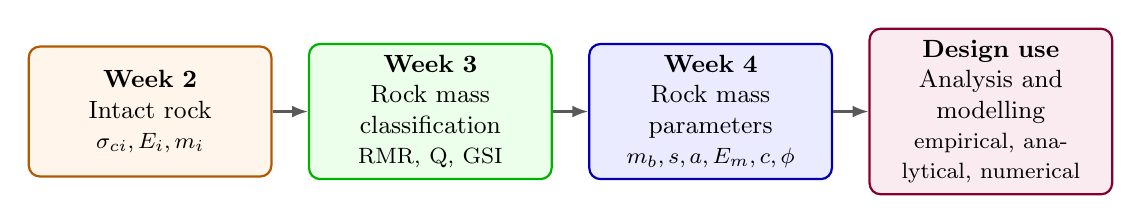
\begin{tikzpicture}[node distance=0.45cm, font=\small]

\node[workflowbox=orange] (w2)
{\textbf{Week 2}\\Intact rock\\
\footnotesize \(\sigma_{ci}, E_i, m_i\)};

\node[workflowbox=green, right=of w2] (w3)
{\textbf{Week 3}\\Rock mass classification\\
\footnotesize RMR, Q, GSI};

\node[workflowbox=blue, right=of w3] (w4)
{\textbf{Week 4}\\Rock mass parameters\\
\footnotesize \(m_b,s,a,E_m,c,\phi\)};

\node[workflowbox=purple, right=of w4] (design)
{\textbf{Design use}\\Analysis and modelling\\
\footnotesize empirical, analytical, numerical};

\draw[workflowarrow] (w2) -- (w3);
\draw[workflowarrow] (w3) -- (w4);
\draw[workflowarrow] (w4) -- (design);

\end{tikzpicture}
}
\caption{Week 3 connects intact rock properties to rock mass design parameters.}
\label{fig:week3_design_chain}
\end{figure}

\begin{notebox}[Important transition]
Intact rock strength from laboratory tests cannot be used directly as rock mass strength.
Rock mass classification provides a structured way to account for discontinuities,
weathering, joint condition, groundwater, and stress conditions.
\end{notebox}

% ======================================================================
\section{Rock Mass Classification -- Overview}
% ======================================================================

Rock mass classification systems were developed to:
\begin{itemize}
    \item identify the most significant parameters influencing rock mass behaviour;
    \item divide rock masses into groups of similar engineering behaviour;
    \item provide quantitative data and guidelines for preliminary design;
    \item support communication between engineers and geologists; and
    \item provide input to empirical support systems and rock mass failure criteria.
\end{itemize}

Key contributors and systems include:
\begin{itemize}
    \item Terzaghi (1946): Rock Load Factor;
    \item Bieniawski (1973, 1989): Rock Mass Rating (RMR);
    \item Barton et al.\ (1974): Q-system;
    \item Hoek et al.\ (1994--1995): Geological Strength Index (GSI);
    \item Molinda and Mark (1994): Coal Mine Roof Rating (CMRR).
\end{itemize}

\begin{keybox}[Classification is not calculation only]
Rock mass classification requires both numerical calculation and geological judgement.
Students must justify the selected ratings, not only report final RMR, Q, or GSI values.
\end{keybox}

% ======================================================================
\section{Classification Workflow}
% ======================================================================

The recommended workflow for Week 3 is shown in Figure~\ref{fig:classification_workflow}.

\begin{figure}[H]
\centering
\resizebox{\textwidth}{!}{%
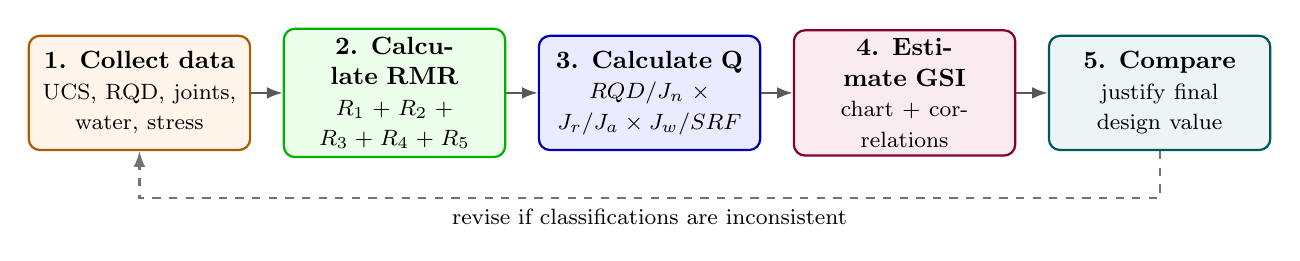
\begin{tikzpicture}[node distance=0.4cm, font=\small]

\node[smallworkflowbox=orange] (data)
{\textbf{1. Collect data}\\
\footnotesize UCS, RQD, joints, water, stress};

\node[smallworkflowbox=green, right=of data] (rmr)
{\textbf{2. Calculate RMR}\\
\footnotesize \(R_1+R_2+R_3+R_4+R_5\)};

\node[smallworkflowbox=blue, right=of rmr] (q)
{\textbf{3. Calculate Q}\\
\footnotesize \(RQD/J_n \times J_r/J_a \times J_w/SRF\)};

\node[smallworkflowbox=purple, right=of q] (gsi)
{\textbf{4. Estimate GSI}\\
\footnotesize chart + correlations};

\node[smallworkflowbox=teal, right=of gsi] (check)
{\textbf{5. Compare}\\
\footnotesize justify final design value};

\draw[workflowarrow] (data) -- (rmr);
\draw[workflowarrow] (rmr) -- (q);
\draw[workflowarrow] (q) -- (gsi);
\draw[workflowarrow] (gsi) -- (check);

\draw[feedbackarrow] (check.south) -- ++(0,-0.6) -| node[pos=0.25,below,font=\footnotesize]
{revise if classifications are inconsistent} (data.south);

\end{tikzpicture}
}
\caption{Recommended rock mass classification workflow.}
\label{fig:classification_workflow}
\end{figure}

\begin{warnbox}[Do not force all systems to agree]
RMR, Q, and GSI measure related but not identical aspects of rock mass quality.
Differences between them are not necessarily mistakes. A good report explains why
the values differ and selects a defensible design value.
\end{warnbox}

% ======================================================================
\section{Rock Mass Rating (RMR) System}
% ======================================================================

The RMR system of Bieniawski (1989) is based on five parameters:
\[
\text{RMR} = R_1 + R_2 + R_3 + R_4 + R_5
\]
where:
\begin{itemize}
    \item \(R_1\) = intact rock strength rating;
    \item \(R_2\) = RQD rating;
    \item \(R_3\) = discontinuity spacing rating;
    \item \(R_4\) = discontinuity condition rating;
    \item \(R_5\) = groundwater rating.
\end{itemize}

\begin{notebox}[Basic RMR vs adjusted RMR]
In Week 3, calculate the \textbf{basic RMR} from the five parameters above.
Orientation adjustment is used later for design applications such as tunnels, slopes,
and foundations. For GSI conversion, use \(RMR_{\text{basic}}\), not an orientation-adjusted RMR.
\end{notebox}

% ----------------------------------------------------------------------
\subsection{R1: Strength of Intact Rock Material}

This rating is based on uniaxial compressive strength or point load index.

\begin{table}[H]
\centering
\small
\begin{tabularx}{0.85\textwidth}{l l c}
\toprule
\textbf{Point Load \(I_{s(50)}\) (MPa)} & \textbf{UCS (MPa)} & \textbf{Rating} \\
\midrule
\(>10\) & \(>250\) & 15 \\
4--10 & 100--250 & 12 \\
2--4 & 50--100 & 7 \\
1--2 & 25--50 & 4 \\
-- & 5--25 & 2 \\
-- & 1--5 & 1 \\
-- & \(<1\) & 0 \\
\bottomrule
\end{tabularx}
\caption{RMR rating for intact rock strength.}
\label{tab:rmr_strength}
\end{table}

% ----------------------------------------------------------------------
\subsection{R2: Rock Quality Designation (RQD)}

\[
\text{RQD} =
\frac{
\sum \text{length of sound core pieces} > 100~\text{mm}
}
{\text{total core run length}}
\times 100\%
\]

\begin{table}[H]
\centering
\small
\begin{tabular}{c c l}
\toprule
\textbf{RQD (\%)} & \textbf{Rating} & \textbf{Description} \\
\midrule
90--100 & 20 & Excellent \\
75--90 & 17 & Good \\
50--75 & 13 & Fair \\
25--50 & 8 & Poor \\
\(<25\) & 3 & Very poor \\
\bottomrule
\end{tabular}
\caption{RMR rating for RQD.}
\label{tab:rmr_rqd}
\end{table}

\begin{warnbox}[RQD is not strength]
RQD is a geometric index. It describes the percentage of core pieces longer than
100 mm. It does not directly measure joint roughness, joint infilling, shear strength,
or deformability.
\end{warnbox}

% ----------------------------------------------------------------------
\subsection{R3: Spacing of Discontinuities}

\begin{table}[H]
\centering
\small
\begin{tabular}{c c}
\toprule
\textbf{Joint spacing (m)} & \textbf{Rating} \\
\midrule
\(>2\) & 20 \\
0.6--2 & 15 \\
0.2--0.6 & 10 \\
0.06--0.2 & 8 \\
\(<0.06\) & 5 \\
\bottomrule
\end{tabular}
\caption{RMR rating for discontinuity spacing.}
\label{tab:rmr_spacing}
\end{table}

If joint spacing is not directly measured, it may be estimated from RQD using the
Priest--Hudson relationship:
\[
RQD = 110.4 - 3.68\lambda
\qquad
(6 < \lambda < 16)
\]
where \(\lambda\) is the joint frequency in joints per metre.

The average joint spacing is then:
\[
s = \frac{1}{\lambda}
\]

\begin{calcbox}[Example calculation]
If \(RQD = 68\%\), then:
\[
\lambda = \frac{110.4 - 68}{3.68} = 11.52~\text{joints/m}
\]
\[
s = \frac{1}{11.52}=0.087~\text{m}
\]
This spacing would fall in the 0.06--0.2 m category.
\end{calcbox}

\begin{warnbox}[Priest--Hudson validity range]
The linear approximation \(RQD = 110.4 - 3.68\lambda\) is only valid for
\(6 < \lambda < 16\), approximately corresponding to RQD values between 51\% and 88\%.
For very poor rock, use this only as a rough guide and explain the uncertainty.
\end{warnbox}

% ----------------------------------------------------------------------
\subsection{R4: Condition of Discontinuities}

\begin{table}[H]
\centering
\small
\begin{tabularx}{\textwidth}{Y c}
\toprule
\textbf{Condition description} & \textbf{Rating} \\
\midrule
Very rough surfaces, not continuous, no separation, unweathered wall rock & 30 \\
Slightly rough surfaces, separation \(<1\) mm, slightly weathered walls & 25 \\
Slightly rough surfaces, separation \(<1\) mm, highly weathered walls & 20 \\
Slickensided surfaces OR gouge \(<5\) mm thick OR separation 1--5 mm, continuous & 10 \\
Soft gouge \(>5\) mm thick OR separation \(>5\) mm, continuous & 0 \\
\bottomrule
\end{tabularx}
\caption{RMR rating for discontinuity condition.}
\label{tab:rmr_condition}
\end{table}

\begin{notebox}[Use the most representative condition]
If the joint description contains mixed features, choose the rating that best represents
the likely engineering behaviour and justify the decision. Do not simply choose the most
favourable description.
\end{notebox}

% ----------------------------------------------------------------------
\subsection{R5: Groundwater Conditions}

\begin{table}[H]
\centering
\small
\begin{tabularx}{\textwidth}{l l l c}
\toprule
\textbf{Inflow per 10 m tunnel (L/min)} & \textbf{\(u/\sigma_1\)} & \textbf{General condition} & \textbf{Rating} \\
\midrule
None & 0 & Completely dry & 15 \\
\(<10\) & 0--0.1 & Damp & 10 \\
10--25 & 0.1--0.2 & Wet & 7 \\
25--125 & 0.2--0.5 & Dripping & 4 \\
\(>125\) & \(>0.5\) & Flowing & 0 \\
\bottomrule
\end{tabularx}
\caption{RMR rating for groundwater.}
\label{tab:rmr_groundwater}
\end{table}

% ----------------------------------------------------------------------
\subsection{Rock Mass Classes Based on RMR}

\begin{table}[H]
\centering
\small
\begin{tabular}{c c l c c}
\toprule
\textbf{RMR} & \textbf{Class} & \textbf{Description} & \textbf{Cohesion (kPa)} & \textbf{Friction angle} \\
\midrule
81--100 & I & Excellent & \(>400\) & \(>45^\circ\) \\
61--80  & II & Good      & 300--400 & 35--45\(^{\circ}\) \\
41--60  & III & Fair      & 200--300 & 25--35\(^{\circ}\) \\
21--40  & IV & Poor      & 100--200 & 15--25\(^{\circ}\) \\
\(<20\) & V & Very poor & \(<100\) & \(<15^\circ\) \\
\bottomrule
\end{tabular}
\caption{Rock mass classes based on RMR.}
\label{tab:rmr_classes}
\end{table}

% ======================================================================
\section{NGI Q-System}
% ======================================================================

The Q-system of Barton et al.\ (1974) is defined as:
\[
Q =
\frac{RQD}{J_n}
\times
\frac{J_r}{J_a}
\times
\frac{J_w}{SRF}
\]

The three terms have physical meaning:
\[
\frac{RQD}{J_n} = \text{block size}
\]
\[
\frac{J_r}{J_a} = \text{inter-block shear strength}
\]
\[
\frac{J_w}{SRF} = \text{active stress and water effect}
\]

\begin{notebox}[RQD is entered as a percentage]
Use \(RQD=70\), not \(0.70\). A common error is to enter the decimal form, which
makes the Q-value 100 times too small.
\end{notebox}

% ----------------------------------------------------------------------
\subsection{Joint Set Number \(J_n\)}

\begin{table}[H]
\centering
\small
\begin{tabularx}{0.85\textwidth}{Y c}
\toprule
\textbf{Joint sets} & \textbf{\(J_n\)} \\
\midrule
Massive, no or few joints & 0.5--1 \\
One joint set & 2 \\
One joint set plus random joints & 3 \\
Two joint sets & 4 \\
Two joint sets plus random joints & 6 \\
Three joint sets & 9 \\
Three joint sets plus random joints & 12 \\
Four or more joint sets, heavily jointed & 15 \\
Crushed rock, earthlike & 20 \\
\bottomrule
\end{tabularx}
\caption{Joint set number \(J_n\).}
\label{tab:jn}
\end{table}

% ----------------------------------------------------------------------
\subsection{Joint Roughness Number \(J_r\)}

\begin{table}[H]
\centering
\small
\begin{tabularx}{0.85\textwidth}{Y c}
\toprule
\textbf{Description} & \textbf{\(J_r\)} \\
\midrule
Discontinuous joints & 4 \\
Rough or irregular, undulating & 3 \\
Smooth, undulating & 2 \\
Slickensided, undulating & 1.5 \\
Rough or irregular, planar & 1.5 \\
Smooth, planar & 1 \\
Slickensided, planar & 0.5 \\
\bottomrule
\end{tabularx}
\caption{Joint roughness number \(J_r\).}
\label{tab:jr}
\end{table}

% ----------------------------------------------------------------------
\subsection{Joint Alteration Number \(J_a\)}

\begin{table}[H]
\centering
\footnotesize
\begin{tabularx}{\textwidth}{Y c c}
\toprule
\textbf{Description} & \textbf{Residual friction angle} & \textbf{\(J_a\)} \\
\midrule
\multicolumn{3}{l}{\textbf{(a) Rock-wall contact, no mineral fillings, only coatings}} \\
Tightly healed, hard, non-softening, impermeable filling & -- & 0.75 \\
Unaltered joint walls, surface staining only & 25--35\(^{\circ}\) & 1 \\
Slightly altered, non-softening mineral coating, sandy particles & 25--30\(^{\circ}\) & 2 \\
Silty- or sandy-clay coatings, small clay fraction, non-softening & 20--25\(^{\circ}\) & 3 \\
Softening or low-friction mineral coatings & 8--16\(^{\circ}\) & 4 \\
\midrule
\multicolumn{3}{l}{\textbf{(b) Rock-wall contact before 10 cm shear, thin fillings}} \\
Sandy particles, clay-free disintegrated rock & 25--30\(^{\circ}\) & 4 \\
Strongly over-consolidated, non-softening clay fillings & 16--24\(^{\circ}\) & 6 \\
Medium or low over-consolidation, softening clay fillings & 12--16\(^{\circ}\) & 8 \\
Swelling clay fillings & 6--12\(^{\circ}\) & 8--12 \\
\midrule
\multicolumn{3}{l}{\textbf{(c) No rock-wall contact when sheared, thick fillings}} \\
Zones of disintegrated or crushed rock, strongly over-consolidated & 16--24\(^{\circ}\) & 6 \\
Zones of clay, medium or low over-consolidation & 12--16\(^{\circ}\) & 8 \\
Zones of clay, swelling clay & 6--12\(^{\circ}\) & 8--12 \\
Thick continuous zones of clay, strongly over-consolidated & 12--16\(^{\circ}\) & 10 \\
Thick continuous zones of clay, medium to low over-consolidation & 12--16\(^{\circ}\) & 13 \\
Thick continuous zones with swelling clay & 6--12\(^{\circ}\) & 13--20 \\
\bottomrule
\end{tabularx}
\caption{Joint alteration number \(J_a\).}
\label{tab:ja}
\end{table}

% ----------------------------------------------------------------------
\subsection{Joint Water Reduction Factor \(J_w\)}

\begin{table}[H]
\centering
\small
\begin{tabularx}{\textwidth}{c Y c c}
\toprule
\textbf{Code} & \textbf{Conditions} & \textbf{Pressure (kg/cm\(^2\))} & \textbf{\(J_w\)} \\
\midrule
A & Dry excavations or minor inflow & \(<1\) & 1.0 \\
B & Medium inflow, occasional outwash of joint fillings & 1--2.5 & 0.66 \\
C & Jet inflow or high pressure in competent rock & 2.5--10 & 0.5 \\
D & Large inflow or high pressure, considerable outwash & 2.5--10 & 0.33 \\
E & Exceptionally high inflow, decaying with time & \(>10\) & 0.2--0.1 \\
F & Exceptionally high inflow, continuing without decay & \(>10\) & 0.1--0.05 \\
\bottomrule
\end{tabularx}
\caption{Joint water reduction factor \(J_w\).}
\label{tab:jw}
\end{table}

% ----------------------------------------------------------------------
\subsection{Stress Reduction Factor (SRF)}
\label{sec:srf}

The SRF accounts for weakness zones, stress problems, squeezing, and swelling conditions.
It is one of the most judgement-sensitive parts of the Q-system.

\begin{table}[H]
\centering
\footnotesize
\begin{tabularx}{\textwidth}{Y c}
\toprule
\textbf{Description} & \textbf{SRF} \\
\midrule
\multicolumn{2}{l}{\textbf{(a) Weakness zones intersecting the excavation}} \\
Multiple weakness zones with clay, very loose surrounding rock & 10 \\
Multiple shear zones in competent clay-free rock & 7.5 \\
Single weak zone with or without clay, depth \(\leq 50\) m & 5.0 \\
Loose, open joints, heavily jointed or ``sugar cube'' rock mass & 5.0 \\
Single weak zone with or without clay, depth \(>50\) m & 2.5 \\
\midrule
\multicolumn{2}{l}{\textbf{(b) Competent rock, stress problems}} \\
Low stress, near surface, open joints, \(\sigma_{ci}/\sigma_1^{IS} > 200\) & 2.5 \\
Medium stress, favourable conditions, \(\sigma_{ci}/\sigma_1^{IS}=200\)--10 & 1.0 \\
High stress, very tight structure, \(\sigma_{ci}/\sigma_1^{IS}=10\)--5 & 0.5--2 \\
Moderate spalling/slabbing, \(\sigma_{ci}/\sigma_1^{IS}=5\)--3 & 5--50 \\
Spalling or rock burst, \(\sigma_{ci}/\sigma_1^{IS}=3\)--2 & 50--200 \\
Heavy rock burst, \(\sigma_{ci}/\sigma_1^{IS}<2\) & 200--400 \\
\midrule
\multicolumn{2}{l}{\textbf{(c) Squeezing rock}} \\
Mild squeezing, \(\sigma_{\theta}/\sigma_c = 1\)--5 & 5--10 \\
Heavy squeezing, \(\sigma_{\theta}/\sigma_c > 5\) & 10--20 \\
\midrule
\multicolumn{2}{l}{\textbf{(d) Swelling rock}} \\
Mild swelling & 5--10 \\
Heavy swelling & 10--15 \\
\bottomrule
\end{tabularx}
\caption{Stress Reduction Factor (SRF).}
\label{tab:srf}
\end{table}

\begin{warnbox}[Choosing the correct SRF category]
Category (b) applies when the rock mass is competent and the ratio
\(\sigma_{ci}/\sigma_1^{IS}\) can be meaningfully calculated.

Here:
\[
\sigma_1^{IS}=\text{maximum in-situ principal stress}
\]
not the Hoek--Brown failure stress \(\sigma_1^f\).

Category (a) applies when the excavation intersects weakness zones, heavily jointed zones,
or poorly interlocked rock, regardless of stress level.
\end{warnbox}

\begin{notebox}[Connection to Week 2 notation]
In Week 2, \(\sigma_1^{IS}\) was used for the maximum in-situ stress demand, while
\(\sigma_1^f\) was used for the major principal stress at failure from Hoek--Brown.
For SRF category (b), use \(\sigma_1^{IS}\), not \(\sigma_1^f\).
\end{notebox}

% ----------------------------------------------------------------------
\subsection{Rock Mass Quality Based on Q}

\begin{table}[H]
\centering
\small
\begin{tabular}{c l}
\toprule
\textbf{Q-value} & \textbf{Rock mass quality} \\
\midrule
\(>400\) & Exceptionally good \\
100--400 & Extremely good \\
40--100 & Very good \\
10--40 & Good \\
4--10 & Fair \\
1--4 & Poor \\
0.1--1 & Very poor \\
0.01--0.1 & Extremely poor \\
\(<0.01\) & Exceptionally poor \\
\bottomrule
\end{tabular}
\caption{Rock mass quality based on Q-value.}
\label{tab:q_quality}
\end{table}

% ======================================================================
\section{Geological Strength Index (GSI)}
% ======================================================================

GSI describes rock mass structure and joint surface condition. It is used directly in
the generalised Hoek--Brown criterion in Week~4.

\begin{keybox}[What GSI should represent]
GSI should reflect the \textbf{geological structure} and \textbf{joint surface condition} of
the rock mass. It should not directly include groundwater, excavation orientation, or
temporary construction effects.
\end{keybox}

% ----------------------------------------------------------------------
\subsection{Structure Descriptions}

\begin{itemize}
    \item \textbf{Intact or massive}: intact rock specimens, few widely spaced discontinuities.
    \item \textbf{Blocky}: well interlocked, cubical blocks formed by approximately three joint sets.
    \item \textbf{Very blocky}: interlocked, partially disturbed, multifaceted angular blocks.
    \item \textbf{Blocky/disturbed/seamy}: folded or faulted rock with many intersecting discontinuities.
    \item \textbf{Disintegrated}: poorly interlocked, heavily broken mixture of rock fragments.
    \item \textbf{Laminated/sheared}: lack of blockiness due to weak foliation, schistosity, or shearing.
\end{itemize}

% ----------------------------------------------------------------------
\subsection{Joint Surface Condition}

\begin{itemize}
    \item \textbf{Very good}: very rough, fresh, unweathered surfaces.
    \item \textbf{Good}: rough, slightly weathered, iron-stained surfaces.
    \item \textbf{Fair}: smooth, moderately weathered and altered surfaces.
    \item \textbf{Poor}: slickensided, highly weathered surfaces with compact coatings or fillings.
    \item \textbf{Very poor}: slickensided, highly weathered surfaces with soft clay coatings or fillings.
\end{itemize}

% ----------------------------------------------------------------------
\subsection{Chart-Based GSI Estimation}

Chart-based GSI estimation uses two judgements:
\[
\text{Rock mass structure}
\quad + \quad
\text{Joint surface condition}
\quad \rightarrow \quad
\text{GSI range}
\]

\begin{notebox}[Recommended reporting style]
Do not report only one GSI number. State the descriptive basis, for example:

``The rock mass is interpreted as blocky to very blocky, with slightly rough but highly
weathered joint surfaces. Therefore, a GSI range of approximately XX--YY is considered
reasonable. A representative value of XX is adopted for Week 4 calculations.''
\end{notebox}

% ----------------------------------------------------------------------
\subsection{Empirical GSI Correlations}

\subsubsection{GSI from RMR}

\[
\boxed{\text{GSI}=RMR_{\text{basic}}-5}
\]

where \(RMR_{\text{basic}}\) is the RMR calculated with:
\begin{itemize}
    \item groundwater rating set to 15, corresponding to completely dry conditions;
    \item orientation adjustment set to 0.
\end{itemize}

If the calculated RMR includes actual groundwater rating \(R_5\), then:
\[
RMR_{\text{basic}} = RMR - R_5 + 15
\]
and:
\[
\text{GSI} = RMR_{\text{basic}} - 5
\]

\begin{calcbox}[Example]
If:
\[
RMR = 60,\qquad R_5=7
\]
then:
\[
RMR_{\text{basic}} = 60 - 7 + 15 = 68
\]
\[
GSI = 68 - 5 = 63
\]
\end{calcbox}

\begin{warnbox}[Do not use raw RMR directly for GSI]
A common error is:
\[
GSI = RMR - 5
\]
without correcting the groundwater rating. This double-counts the groundwater penalty.
GSI should describe rock mass structure and joint surface condition, not groundwater.
\end{warnbox}

\subsubsection{Other Empirical Correlations}

Two additional empirical correlations are:
\[
GSI = 1.5J_{\text{cond89}} + \frac{RQD}{2}
\]
and:
\[
GSI =
\frac{52(J_r/J_a)}
{1+(J_r/J_a)}
+
\frac{RQD}{2}
\]

where \(J_{\text{cond89}}\) is the RMR joint condition rating \(R_4\), not the Q-system
joint roughness number \(J_r\).

\begin{warnbox}[Symbol caution]
\(J_{\text{cond89}}\) is the RMR joint condition rating. It is not the same as \(J_r\) in
the Q-system. Mixing these two symbols gives incorrect GSI values.
\end{warnbox}

% ======================================================================
\section{How to Select a Final GSI Value}
% ======================================================================

Students should compare:
\begin{itemize}
    \item chart-based GSI;
    \item GSI from \(RMR_{\text{basic}}-5\);
    \item GSI from \(1.5J_{\text{cond89}}+RQD/2\);
    \item GSI from the \(J_r/J_a\) correlation.
\end{itemize}

\begin{figure}[H]
\centering
\resizebox{0.95\textwidth}{!}{%
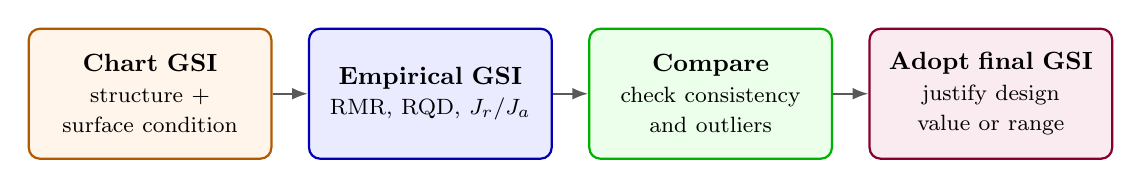
\begin{tikzpicture}[node distance=0.45cm, font=\small]

\node[workflowbox=orange] (chart)
{\textbf{Chart GSI}\\
\footnotesize structure + surface condition};

\node[workflowbox=blue, right=of chart] (corr)
{\textbf{Empirical GSI}\\
\footnotesize RMR, RQD, \(J_r/J_a\)};

\node[workflowbox=green, right=of corr] (compare)
{\textbf{Compare}\\
\footnotesize check consistency and outliers};

\node[workflowbox=purple, right=of compare] (select)
{\textbf{Adopt final GSI}\\
\footnotesize justify design value or range};

\draw[workflowarrow] (chart) -- (corr);
\draw[workflowarrow] (corr) -- (compare);
\draw[workflowarrow] (compare) -- (select);

\end{tikzpicture}
}
\caption{Workflow for selecting a defensible GSI value.}
\label{fig:gsi_selection}
\end{figure}

\begin{keybox}[Preferred approach]
Use the chart-based GSI as the primary geological judgement. Use empirical correlations
as checks. If the values differ significantly, explain why and adopt a conservative but
reasonable design value.
\end{keybox}

% ======================================================================
\section{Project Input Data for Assignment 1}
% ======================================================================

The following table summarises the key rock mass information for Assignment 1.
Students must use the full project descriptions in the assignment brief when assigning
ratings.

\begin{table}[H]
\centering
\scriptsize
\begin{tabularx}{\textwidth}{l Y Y Y Y}
\toprule
\textbf{Parameter} & \textbf{Granite} & \textbf{Sandstone} & \textbf{Mudstone} & \textbf{Limestone} \\
\midrule
\(\sigma_{ci}\) (MPa) & 265 & 110 & 27 & 85 \\
\(I_{s(50)}\) (MPa) & 12.2 & 5.3 & 2.3 & 5.0 \\
RQD (\%) & 70 & 68 & 38 & 52 \\
Joint condition & Tight, closed, very rough, undulating, unweathered & Slightly rough, highly weathered, not separated & Slickensided and planar, aperture 1--2 mm & Smooth, undulating, slightly weathered, clay-filled, aperture 1--2 mm \\
Joint sets / structure & Two joint sets from core observations & One sub-horizontal and one sub-vertical set & Poorly interlocked, heavily jointed, more than four sets & One joint set, spacing approximately 0.15 m \\
Groundwater & Dry & Medium inflow expected & Dripping at outcrop; medium inflow expected & Groundwater table 10 m below surface \\
Depth (m) & 780 & 450 & 100 & 80 \\
Stress ratio \(K\) & 3.2 & 1.8 & 1.0 & 2.0 \\
\bottomrule
\end{tabularx}
\caption{Summary of Assignment 1 rock mass information for Week 3 classification.}
\label{tab:assignment1_week3_data}
\end{table}

\begin{notebox}[Do not treat this table as the full answer]
The table summarises key information only. Students still need to assign ratings,
show calculations, and justify decisions using the detailed assignment description.
\end{notebox}

% ======================================================================
\section{Recommended Calculation Tables for Student Reports}
% ======================================================================

\subsection{RMR Calculation Template}

\begin{table}[H]
\centering
\small
\begin{tabularx}{\textwidth}{l Y c Y}
\toprule
\textbf{RMR parameter} & \textbf{Description/value} & \textbf{Rating} & \textbf{Justification} \\
\midrule
\(R_1\): Intact strength &  &  &  \\
\(R_2\): RQD &  &  &  \\
\(R_3\): Joint spacing &  &  &  \\
\(R_4\): Joint condition &  &  &  \\
\(R_5\): Groundwater &  &  &  \\
\midrule
\multicolumn{2}{r}{\textbf{Total RMR}} &  &  \\
\bottomrule
\end{tabularx}
\caption{Suggested RMR calculation table for each rock type.}
\label{tab:rmr_template}
\end{table}

\subsection{Q-System Calculation Template}

\begin{table}[H]
\centering
\small
\begin{tabularx}{0.85\textwidth}{l Y c}
\toprule
\textbf{Parameter} & \textbf{Description/value} & \textbf{Adopted value} \\
\midrule
RQD &  &  \\
\(J_n\) &  &  \\
\(J_r\) &  &  \\
\(J_a\) &  &  \\
\(J_w\) &  &  \\
SRF &  &  \\
\midrule
\multicolumn{2}{r}{\textbf{Q-value}} &  \\
\bottomrule
\end{tabularx}
\caption{Suggested Q-system calculation table for each rock type.}
\label{tab:q_template}
\end{table}

\subsection{GSI Comparison Template}

\begin{table}[H]
\centering
\small
\begin{tabularx}{\textwidth}{l c Y}
\toprule
\textbf{Method} & \textbf{GSI value/range} & \textbf{Comment} \\
\midrule
Chart-based GSI &  & Based on rock structure and surface condition \\
\(RMR_{\text{basic}}-5\) &  & Groundwater corrected \\
\(1.5J_{\text{cond89}}+RQD/2\) &  & Uses RMR joint condition rating \\
\(J_r/J_a\) correlation &  & Uses Q-system roughness and alteration numbers \\
\midrule
\textbf{Adopted GSI} &  & Justify final value or range \\
\bottomrule
\end{tabularx}
\caption{Suggested GSI comparison table for each rock type.}
\label{tab:gsi_template}
\end{table}

% ======================================================================
\section{Assignment 1 Tasks: Week 3 Component}
% ======================================================================

\begin{enumerate}
    \item \textbf{Determine RMR for each rock type.}
    Create a table showing each parameter, its value, the assigned rating, and a brief
    justification.

    \item \textbf{Calculate the Q-value for each rock type.}
    Clearly define all input parameters:
    \[
    RQD,\quad J_n,\quad J_r,\quad J_a,\quad J_w,\quad SRF
    \]
    and show the calculation.

    \item \textbf{Estimate GSI using the chart-based descriptive method.}
    Provide a short justification based on rock mass structure and joint surface condition.

    \item \textbf{Estimate GSI using empirical correlations.}
    For the RMR-based correlation, show the \(RMR_{\text{basic}}\) correction explicitly.
    Compare all empirical values with the chart-based GSI and discuss discrepancies.
\end{enumerate}

\begin{calcbox}[Minimum reporting expectation]
For each rock type, the report should include:
\begin{itemize}
    \item one RMR calculation table;
    \item one Q-system calculation table;
    \item one GSI comparison table;
    \item a short paragraph explaining the adopted GSI and uncertainty.
\end{itemize}
\end{calcbox}

% ======================================================================
\section{Common Mistakes}
% ======================================================================

\begin{errbox}[Common mistakes in Week 3]
\begin{itemize}
    \item Entering RQD as 0.70 instead of 70 in the Q-system.
    \item Using raw RMR directly for GSI without correcting groundwater.
    \item Confusing \(J_{\text{cond89}}\) with \(J_r\).
    \item Selecting SRF category (b) using the Hoek--Brown failure stress \(\sigma_1^f\)
    instead of the maximum in-situ stress \(\sigma_1^{IS}\).
    \item Reporting RMR, Q, or GSI values without explaining rating choices.
    \item Assuming RMR, Q, and GSI must give identical rock mass quality.
    \item Using one optimistic GSI value without considering uncertainty or range.
    \item Forgetting that the Week 3 GSI value becomes a key input for Week 4.
\end{itemize}
\end{errbox}

% ======================================================================
\section{Week 3 Summary}
% ======================================================================

\begin{table}[H]
\centering
\small
\begin{tabularx}{\textwidth}{l Y Y}
\toprule
\textbf{Topic} & \textbf{Key output} & \textbf{Connection to Assignment 1} \\
\midrule
RMR & Basic rock mass rating from five parameters & Classifies rock mass quality and supports GSI estimation \\
Q-system & \(Q = RQD/J_n \times J_r/J_a \times J_w/SRF\) & Provides an independent quality index and support-design basis \\
SRF & Stress and weakness-zone adjustment & Requires correct use of in-situ stress demand \\
GSI chart & Geological judgement from structure and surface condition & Primary input for Week 4 Hoek--Brown rock mass parameters \\
GSI correlations & Empirical checks from RMR, RQD, and Q parameters & Used to compare and justify adopted GSI values \\
Uncertainty & Rating subjectivity and geological variability & Must be discussed in report and carried into Week 4 \\
\bottomrule
\end{tabularx}
\caption{Week 3 summary.}
\label{tab:week3_summary}
\end{table}

\section{Key Takeaways}

\begin{itemize}
    \item Rock mass classification converts geological observations into engineering indices.
    \item RMR, Q, and GSI are related but not interchangeable.
    \item RMR includes strength, RQD, spacing, condition, and groundwater.
    \item  Q-system separates block size, joint shear strength, and active stress/water effects.
    \item GSI should represent rock mass structure and joint surface condition.
    \item \(RMR_{\text{basic}}\), not raw wet RMR, should be used for GSI conversion.
    \item SRF selection requires engineering judgement and correct stress notation.
\end{itemize}

\vspace{1cm}
\noindent\textit{End of Week 3 Study Notes}

\end{document}